% Generated from the editable manuscript diagram.
\documentclass[12pt,border=3pt]{standalone}
\usepackage{tikz}
\usetikzlibrary{arrows.meta,positioning,fit,calc,shapes.geometric}
\tikzset{block/.style={draw=black!65,rounded corners=2pt,align=center,fill=blue!4,inner sep=6pt,font=\small},
 link/.style={-{Latex[length=2mm]},thick},note/.style={align=center,font=\footnotesize}}
\begin{document}
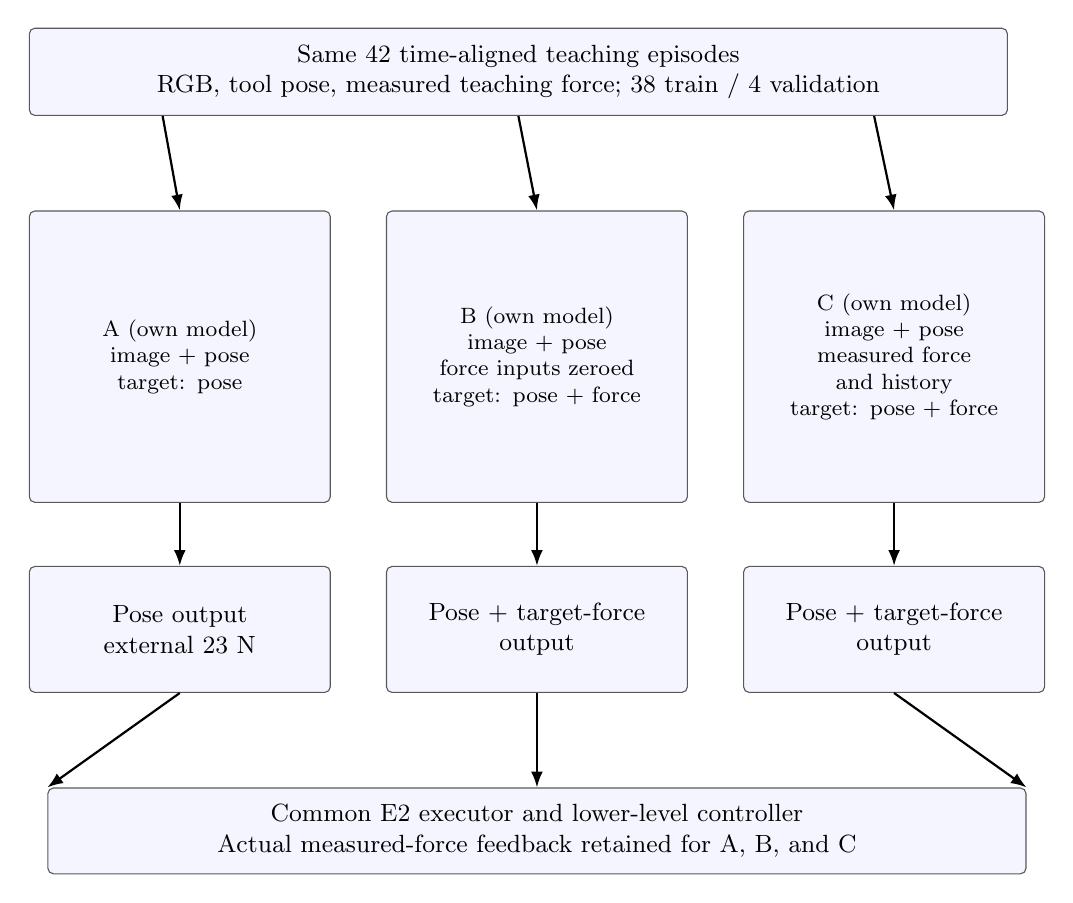
\begin{tikzpicture}[node distance=8mm]
\node[block,text width=120mm] (data) {Same 42 time-aligned teaching episodes\\RGB, tool pose, measured teaching force; 38 train / 4 validation};
\node[block,text width=34mm,font=\footnotesize,minimum height=37mm,below=12mm of data.south west,anchor=north west] (a) {A (own model)\\image + pose\\target: pose};
\node[block,text width=34mm,font=\footnotesize,minimum height=37mm,right=7mm of a] (b) {B (own model)\\image + pose\\force inputs zeroed\\target: pose + force};
\node[block,text width=34mm,font=\footnotesize,minimum height=37mm,right=7mm of b] (c) {C (own model)\\image + pose\\measured force\\and history\\target: pose + force};
\node[block,text width=34mm,minimum height=16mm,below=8mm of a] (ao) {Pose output\\external 23 N};
\node[block,text width=34mm,minimum height=16mm,below=8mm of b] (bo) {Pose + target-force\\output};
\node[block,text width=34mm,minimum height=16mm,below=8mm of c] (co) {Pose + target-force\\output};
\node[block,text width=120mm,below=12mm of bo] (exec) {Common E2 executor and lower-level controller\\Actual measured-force feedback retained for A, B, and C};
\draw[link](data.south west)++(17mm,0)--(a.north);
\draw[link](data.south)--(b.north);
\draw[link](data.south east)++(-17mm,0)--(c.north);
\draw[link](a)--(ao);\draw[link](b)--(bo);\draw[link](c)--(co);
\draw[link](ao.south)--(exec.north west);\draw[link](bo)--(exec);\draw[link](co.south)--(exec.north east);
\end{tikzpicture}
\end{document}
